\documentclass[a4paper]{scrartcl}

\usepackage[utf8]{inputenc}
\usepackage[english]{babel}
\usepackage{lmodern} 
\usepackage[T1]{fontenc}
\usepackage{booktabs}
\usepackage{multirow}
\usepackage{wrapfig}
\usepackage{caption}



% PAKETE
\usepackage{siunitx}
\usepackage{amsmath}
\usepackage{amssymb}
\usepackage{graphicx}
\usepackage{placeins}
\usepackage{longtable}
\usepackage{enumitem}
\usepackage{bbm}



% EINSTELLUNGEN
\sisetup{seperr,repeatunits=false}
\numberwithin{equation}{section}
\numberwithin{figure}{section}
\numberwithin{table}{section}

% EIGENE FUNKTIONEN
\newcommand{\re}{\operatorname{Re}}
\newcommand{\im}{\operatorname{Im}}
\newcommand{\gquote}[1]{\glqq #1 \grqq}

\newcommand{\eq}[2]{\begin{equation}#1\label{#2}\end{equation}}
\newcommand{\eqand}[0]{\hspace{.25cm} \bigwedge \hspace{.25cm}}
\newcommand{\grafik}[2]{\begin{figure}[h]\centering \includegraphics[width=10cm]{#1.eps}  \caption{#2} \label{#1} \end{figure} }
\newcommand{\grafikq}[3]{\begin{figure}[h]\centering \includegraphics[width=10cm]{#1.eps}  \caption[#2]{#3} \label{#1} \end{figure} }
\newcommand{\tbl}[3]{\begin{table}[h]\caption{#1}\label{#2}\begin{center}#3\end{center}\end{table}}
\newcommand{\Abbildung}[1]{\textsl{Abbildung \ref{#1}}}
\newcommand{\AbbildungI}[1]{\textsl{(Abbildung \ref{#1})}}
\newcommand{\Tabelle}[1]{\textsl{Tabelle \ref{#1}}}
\newcommand{\TabelleI}[1]{\textsl{(Tabelle \ref{#1})}}
\newcommand{\Formel}[1]{(\ref{#1})}
\renewcommand{\d}{\mathrm{d}}

\title{Ma 10: Auger- and Electron Energy Loss Spectroscopy}
\subtitle{Tutor: L. Bogner}
\author{Benjamin Huber, Carolin Wille}
\date{October 23, 2011}

\begin{document}
\thispagestyle{empty}
\maketitle
\tableofcontents
\clearpage


\section{Introduction}
In this experiment a aluminium substrate will be analyzed with surface spectroscopial methods. Due to the small penetration depth of the Auger electron spectroscopy (AES) it will be used to detect impurities. After measuring the Auger spectrum of pure Aluminium, the electron enery loss (eel) method will be used to detect plasmons.

\subsection{Cylindrical Mirror Analyzer (CMA)}
The CMA is an apparatus , which selects electrons within a small range of energy $\Delta E$ around a certain energy value $E_0$ from an electron source of various energies. This is performed by two cylinders, where the inner cylinder of radius $r_1$ has two ring-slits for the exit and entrance of the electron beam and a negative potential $V$ is applied to the outer cylinder with radius $r_2$ (Fig. \ref{cma}). 

\begin{figure}[htbp]
\centering
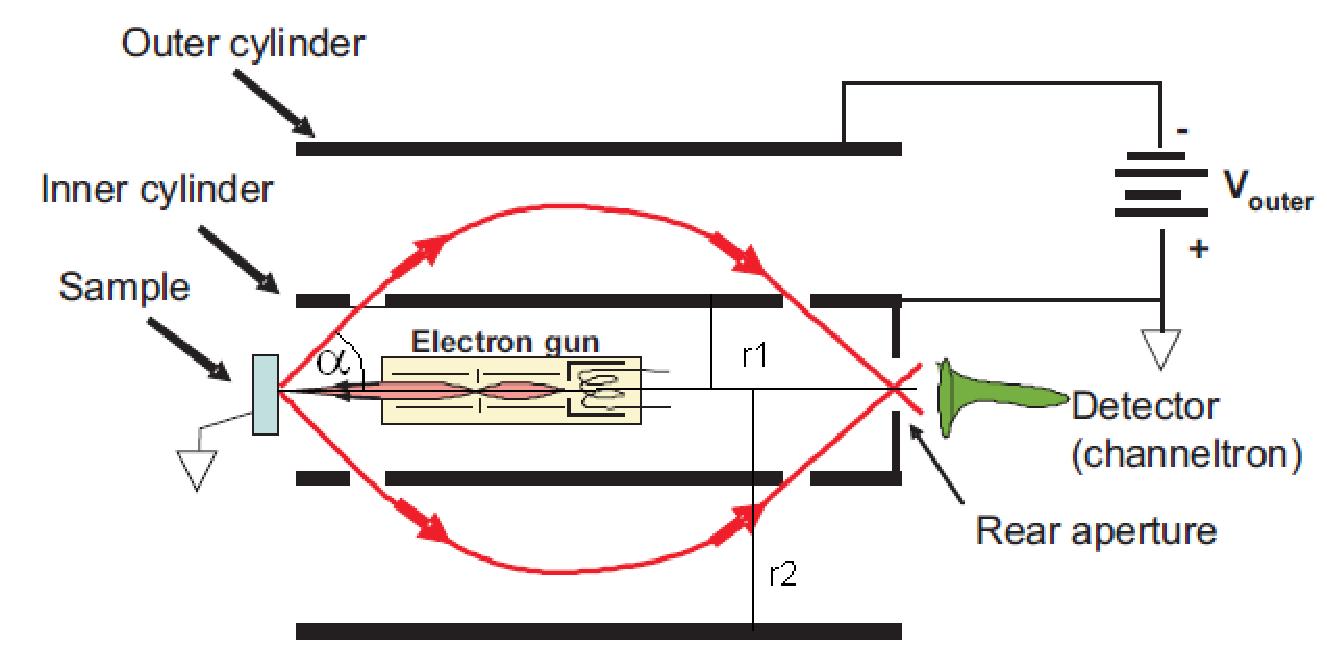
\includegraphics[width=0.6 \textwidth]{cma.pdf}
\caption{\small Schematic cross section of a CMA. \cite{skript}}
\label{cma}
\end{figure}

Therefore, the electrons are bend towards the inner cylinder again. There exist a special emission angle $\alpha=42\degree 18,5 '$, where the focusing properties are eminently better (focus of 2nd order). For CMAs operated at this angle the selected energy value is given by
\eq{E_0 = \frac{1.3099 e}{\log{r_2/r_1}} V \; ,}{E0}
where $e$ is the electron charge. The energy resolution is determined by the angular spread of the emission angle $\Delta \alpha$ (Fig. \ref{cma}) and given by
\eq{\frac{\Delta E}{E_0} = 2.75 \Delta \alpha^3 \; .}{dE} 
%The exact position of the probe in the CMA is very important, as a shift in the probe position $\Delta L$, leads to a shift of the detected peak energy by
%\eq{\Delta E_0 = E_0 \frac{\Delta L}{5.6 r_1} \;.}{dE0}
The current at the detector $I$ is proportional to the number of incoming  electrons $N(E)$. By measuring the voltage $V$, the function $N(E)$ is directly given by \Formel{E0}. However, the characteristic Auger-peaks are easier to detect considering the derivative $\frac{\d N(E)}{\d E}$. This can be achieved by a small sinusoidal modulation of the voltage with amplitude $V_\omega$. % according to
%\eq{V= V_0 + V_\omega \sin \omega t \; . }{}%
The current $I$ can then be expanded in terms of the small perturbation $V_\omega \sin \omega t$ as
\eq{ I = I(V_0) + \frac{\d I}{\d V} V_\omega \sin \omega t + \ldots \; ,}{}
where the derivative $\frac{\d I}{\d V}$ represents the amplitude of the oscillating signal and is proportional to $\frac{\d N(E)}{\d E}$
\eq{\frac{\d I}{\d V} = A_\omega \propto \frac{\d N(E)}{\d E} \; . }{}
This amplitude can be selected and amplified using a lock-in amplifier. 

\subsection{Lock-in Amplifier}
In general the term lock-in amplifier refers to an amplifier, which is operated using an external characteristic signal, that is multiplied with the signal to be amplified, instead of an unspecific amplification. This characteristic external signal is related to the incoming signal, mostly via the frequency. E.g. during a measurement process a signal $S_I$ of known frequency $\omega$ is created according to
\eq{S_I = A_0 + A_\omega \sin \omega t \; . }{SI}
Then an amplification signal $S_A$ of the same phase and frequency is used to amplify the incoming signal and afterwards an integration over a complete period is performed. The out-coming signal $S_O$
%\eq{S_O = \int^\tau_0 S_I S_A \d t }{SA} % 
is then proportional to the amplitude $A_\omega$ of the incoming signal $S_I$
\eq{S_O \propto A_\omega \; .}{}
Therefore, the signal-to-noise relation can be significantly improved, as the constant off-set $A_0$ is almost completely eliminated form the signal.


\subsection{Nomenclature}
The most commonly used nomeclature for the Auger electron spectroskope is based on the quantum number $n$ (K for $n=1$, L for $n=2$...), followed by an index to denote the different possible states for this $n$ (in the order of increasing energy). To fully describe the Auger electron, all three participating states have to be mentioned in this way. 

Alternatively it is possible to simply note the electron configuration at the end of the auger process. In this way $2s^02p^6$ corresponds to $KL_1L_1$ and so on.


\subsection{Expected Transitions}
For aluminum the ionization energy of the K-level is about \SI{1,6}{keV}. Therefore, the typical energy of exciting electrons up to \SI{3}{keV} is sufficient to excite the Auger KLL-transitions, which are the transitions of highest energy. These have an energy range from approximately \SI{1,3}{keV} to \SI{1,4}{keV} and are listed in table \ref{kll}. The LMM transition is also possible and its energy is around \SI{70}{eV} with again a multiplet splitting.

%\begin{figure}[htbp]
%\centering
%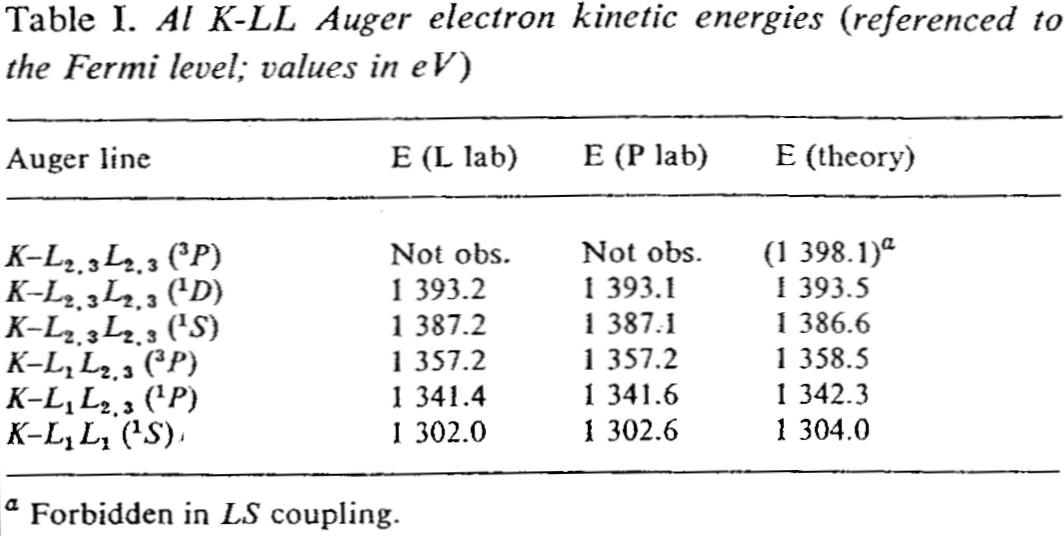
\includegraphics[width=0.6 \textwidth]{referenztab.png}
%% \caption{\small . \cite{paper1}}
%\caption{\small Table taken from \cite{paper}. The first two columns refer to measurements performed by two different experimental groups (bla) and (blub). }
%\label{KLL predict}
%
%\end{figure}

\begin{table}[!h]
\centering

\begin{tabular}{lcc}
\toprule
Auger line & & Theoretical Energy (eV) \\
\midrule
 $KL_{2,3}L_{2,3}$&$(^3P)$  & $(1398.1)^\alpha$ \\
$ KL_{2,3}L_{2,3}$&$(^1D) $ & $1393.5$ \\
$ KL_{2,3}L_{2,3}$&$(^1S)$ & $1386.6 $ \\
$ KL_{1}L_{2,3}$&$(^3P)$ & $1358.5$ \\
$ KL_{1}L_{2,3}$&$(^1P)$ & $1342.3$ \\
$ KL_{1}L_{1}$&$(^1S)$ & $1304.0$ \\
 \bottomrule

\end{tabular}


\caption{\small Theoretical energies \cite{paper} of KLL Auger-Transitions for Aluminum. $^\alpha$: Forbidden due to parity conservation. }
\label{kll}
\end{table}


\subsection{Energy of Auger-Electrons}
The energy balance of the Auger-transition reads
\eq{E(KLL') = E(K) -E(L) - E^{*}(L') \; ,}{EKLL}
where $E(KLL')$ is the energy of the Auger electron stemming from a transition KLL', E(K)/E(L) are the binding energies of the electrons in K/L-level and $E^*(L')$ is the binding energy of the electron in the $L'$ state, where the asterisk denotes, that this energy is altered through the absence of the $K$ and $L$ electron towards.
\eq{E^*(L') = E(L') + C(LL',T) -R \; ,}{E*}
where $C(LL',T)$ stems from the coupling of the two holes in $LL'$, $T$ represents the final state and $R$ is the relaxation energy arising from the reduction of repelling electronic force. 

These formulas hold for free atoms. For an electron, that is emitted from the valence band of a solid the work-function, which gives the minimum energy needed to remove an electron from a solid to the solid surface, has to be taken into account.


\subsection{Plasmons}
The pseudo particle of fermi-gas oscillation is called a plasmon. These plasmons have characteristic energies, depending on the conduction electron density $n$. 
$$E_p = \hbar \underbrace{\sqrt{\frac{ne^2}{m\epsilon_0}}}_{\omega_p}$$
Apart from the more obvious bulk plasmons (three dimensional oscillations in the sample) there are also surface plasmons when a material with positive dielectric constant (vacuum) interface with a material of negative dielectric constant (Al). For Aluminium the bulk and surface plasmons have energies of approximately $15.3 \text{eV}$ and $10.8 \text{eV}$ respectively.
% from [8]? "Comparison of the secondary-e spectrum..."

An electron that excites a plasmon looses one of these characteristic energies and is said to have suffered plasmon loss. It is possible, that one electron suffers plasmon loss several times, leading to a series of equally spaced losses with decreasing intensity.


\subsection{Electron Mean Free Path}
As the mean free path of electrons depends characteristically on the energy of the electrons for a broad range of different materials, the so called universal curve (Fig. \ref{mf}) is very useful in order to analyze the surface sensibility of spectroscopic methods. The minimal lies path exist between \SI{40}{eV} and \SI{100}{eV}. Within this energy range the average penetration depth is below \SI{10}{\AA}. Towards higher electron energies the mean free path increases only slowly and for \SI{1}{keV} is still below \SI{20}{\AA}. Therefore, any electron spectroscopic measurements within this energy range analyses surface properties rather than these of the bulk-solid. 
\begin{figure}[htbp]
\centering
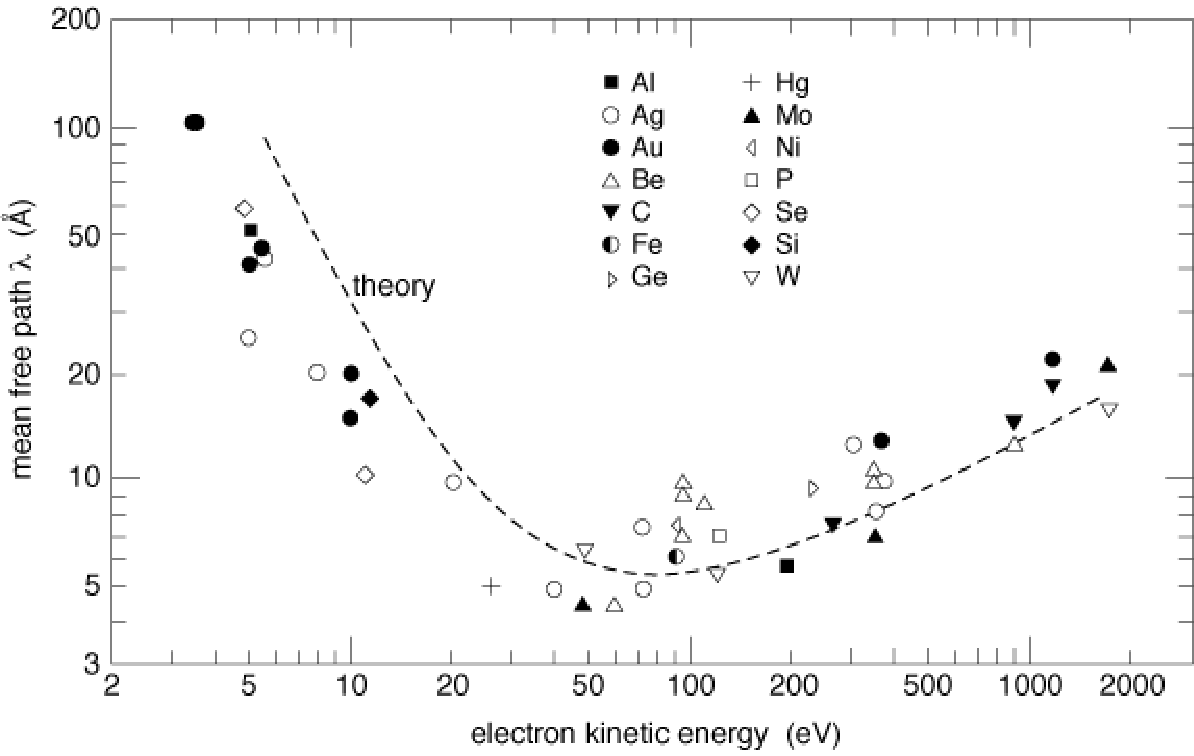
\includegraphics[width=0.5 \textwidth]{meanfree.pdf}
\caption{\small Mean free path of electrons in solids (logarithmic scale). Dots: Measurements. Dashed Line: Calculation. For Aluminium the mean-free path is even smaller then predicted by calculation. \cite{zangwill} }
\label{mf}
\end{figure}


\clearpage
\newpage
\section{Analysis}
\subsection{Oxidization}
Due to the imperfect vacuum in the experimantation chamber, the Al is exposed to oxygen all the time. At the beginning of the measurements this shows as a significant buildup of oxygen atoms at the surface of the sample (see Figure \ref{fig:putz}a). Even though it can be removed very easily mechanically (Fig \ref{fig:putz}b), the constant presence of oxygen causes new oxidation. In the time of about 2 hours at $4.3 \cdot 10^{-8} \text{mbar} \approx 230 \text{L}$ the contamination had already reached more than $50\%$ of the equilibrium level (Fig\ref{fig:putz}c).

\begin{figure}[!p]
        \begin{center}
        \begin{tabular}{l c r}
        		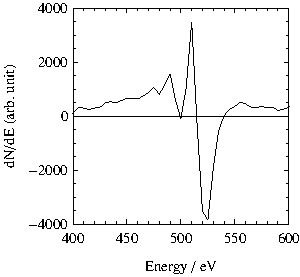
\includegraphics[width=0.31\linewidth]{pic/putz1.pdf}
       	&
       		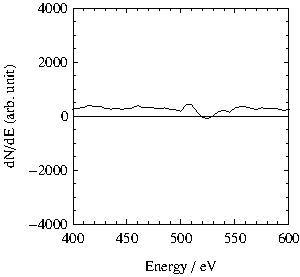
\includegraphics[width=0.31\linewidth]{pic/putz2.pdf}
			&
				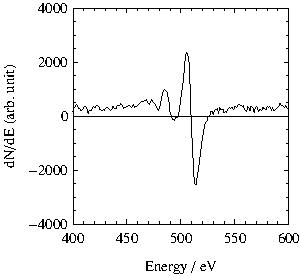
\includegraphics[width=0.31\linewidth]{pic/putzAfter.pdf}
		  \end{tabular}
        \end{center}
        \caption[differential detection rate at the O specific energies]{
			\small Differential detection rate at the oxygen specific energies before cleaning \textbf{(a)}, after cleaning \textbf{(b)} and after the experiments \textbf{(c)}. The characteristic minima are at approximately $(477.8\pm1.0)\text{eV}$, $(494.07\pm0.30)\text{eV}$ and $(514.12\pm0.66)\text{eV}$. Values obtained through the fitting of quadractic functions near the minima.
        }
        \label{fig:putz}
\end{figure}


\subsection{KLL Auger spectrum of Al}
\label{sec:kll}
\begin{figure}[!p]
        \begin{center}
		  \begin{tabular}{l r}
        		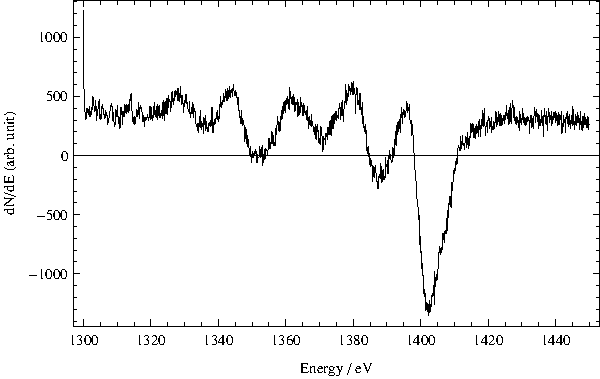
\includegraphics[width=0.48\linewidth]{pic/auger.pdf}
			&
				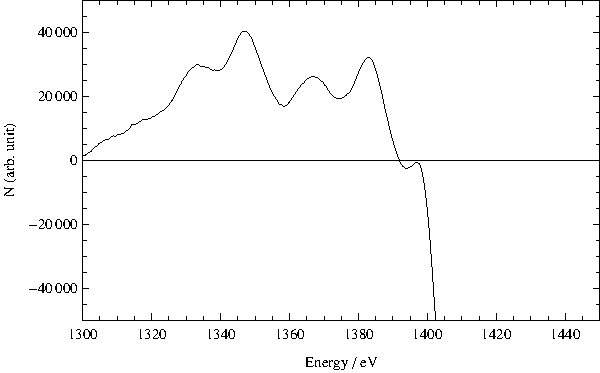
\includegraphics[width=0.48\linewidth]{pic/augerSum.pdf}
        \end{tabular}
        \end{center}
        \caption[(differential) detection rate at the Al specific energies]{
			\small All values obtained by fitting quadractic functions near the minima.
			\textbf{(a)} Measured differential detection rate of Al. Minima at $(1336.07\pm 0.30)\text{eV}$, $(1352.52\pm 0.20)\text{eV}$, $(1370.73\pm 0.32)\text{eV}$, $(1388.32\pm 0.16)\text{eV}$, $(1402.64\pm 0.14)\text{eV}$.
			\textbf{(b)} Integrated version of (a) after substracting an estimated noise level of $~300$. The peaks are at $(1333.64\pm 0.64)\text{eV}$, $(1346.98\pm 0.03)\text{eV}$, $(1366.90\pm 0.05)\text{eV}$, $(1382.81\pm 0.04)\text{eV}$, $(1396.96\pm 0.08)\text{eV}$.
        }
        \label{fig:auger}
\end{figure} 

With the cleaned sample, the differential spectrum of aluminium has its most noteable activity near $1400\text{eV}$. The qualitative form of this region (Fig \ref{fig:auger}) is in very well agreement with the literature (cf. handbook of aes) but quantitavely all values seem to be shifted towards higher energies.

This shift is expected, considering the poor alignment of the sample. A deviation from the perfect position $\Delta x$ will cause a streching of the form
\eq{E' = \lambda (\Delta x) \cdot E,}{}
where $E'$ is the measured and $E$ the actual energy of the electrons (->SOURCE). Assuming the deviation does not change significantly over the time of measurement, we can try to recalibrate our measurements with the known minima in the oxygen spectrum.

The resulting values are (or close to) consistent with the literature, but have a rather large margin of error. Using the last minimum of the Al spectrum to calibrate the spectroscope instead gives better values. While this does not allow to compare the absolut values, the relative spacing between the minima can still be compared and confirmed. Due to the significant improvement in accuracy this last calibration will be used throughout the rest of this work.

\begin{table}[!p]
\centering
\begin{tabular}{ccc}
\toprule
O calibration & Al calibration & literature \\
\midrule
$(1325.1\pm 3.5)$ & $(1329.7\pm 1.2)$ & 1329 \\
$(1341.4\pm 3.5)$ & $(1346.1\pm 1.2)$ & 1345 \\
$(1359.4\pm 3.6)$ & $(1364.2\pm 1.2)$ & 1364 \\
$(1376.9\pm 3.6)$ & $(1381.8\pm 1.2)$ & 1380 \\
$(1391.1\pm 3.6)$ & $(1396.0\pm 1.2)$ & 1396 \\
 \bottomrule
\end{tabular}
\caption{\small Positions of the minima in the differential (dN/dE) aluminium auger spectrum. Values corrected with the information of the oxygen minima or the last aluminium minimum compared to the values in the literature. All values in eV. }
\label{tab:OAlL}
\end{table}

The integrated version of this spectrum shows peaks corresponding to KLL auger effects in aluminium. The resolution is far too bad to allow the identification of all five expected transitions, but with a reference spectrum from \cite{paper} it is possible to identify the 5 most significant peaks. See Table \ref{tab:kll} for more details.

% TODO change to row-table?
\begin{table}[htbp]
\centering
\begin{tabular}{lcc}
\toprule
transition & literature & measurement \\
\midrule
$^1P + B_1$ & 1326.1 & $(1327.3\pm 1.1)$  \\
\midrule
$^1P$ 		& 1341.4 & $(1340.6\pm 1.1)$ \\
\midrule
$^3P$ 		& 1357.2 & \multirow{2}{*}{$(1360.4\pm 1.2)$}  \\
$^1D + B_2$ & 1362.6 & \\
\midrule
$^1D + B_1$ & 1377.9 & $(1376.3\pm 1.2)$ \\
\midrule
$^1D$ 		& 1393.2 & \multirow{2}{*}{$(1390.4\pm 1.2)$}  \\
$^1S$ 	   & 1387.2 & \\
 \bottomrule
\end{tabular}
\caption{\small Characteristic (corrected) energies of the KLL auger spectrum of aluminium, their according transition and the literature value from \cite{}. $+B_{1/2}$ denotes the change in energy due to the interaction with bulk plasmons. Whenever two significant peaks are closer than $7\text{eV}$ they merge, resulting in a single, mean value in the measurements due to the very limited resolution of the used apparatus. }
\label{tab:OAlL}
\end{table}

\subsection{Plasmons}
\label{sec:plas}
The most significant peaks in section \ref{sec:kll} already contained electrons that suffered plasmon loss. These characteristic losses can be measured with electron energy loss spectroscopy. A measurement with higher energy electrons (1keV) shows mainly the bulk plasmons, while a second measurement with weaker electrons (170eV) promises to show surface plasmons more clearly, due to the lower penetration depth.

%TODO noch ein satz zu EEL? backscatter electrons ->

The first measurement (see Fig \ref{fig:plas}b) resulted in a (weighted) mean energy for the bulk plasmons of $B_1 = (15.31\pm 0.54)\text{eV}$. This result is consistent with the two bulk plasmons found in the 170eV measurement (see Fig \ref{fig:plas}a). The single peak in the second measurement corresponding to a surface plasmon results in $S_1 = (11.04\pm 0.20)\text{eV}$. 

\begin{figure}[htbp]
        \begin{center}
		  \begin{tabular}{l r}
        		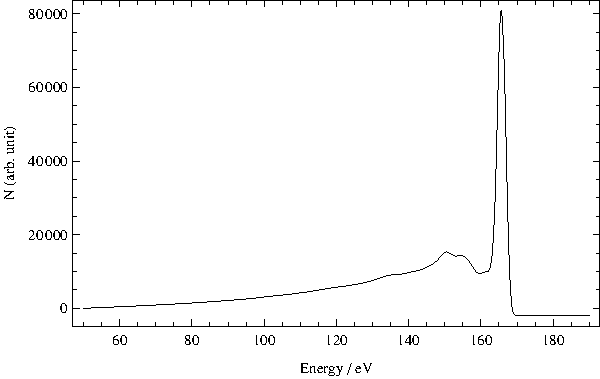
\includegraphics[width=0.48\linewidth]{pic/plasmon200.pdf}
			&
				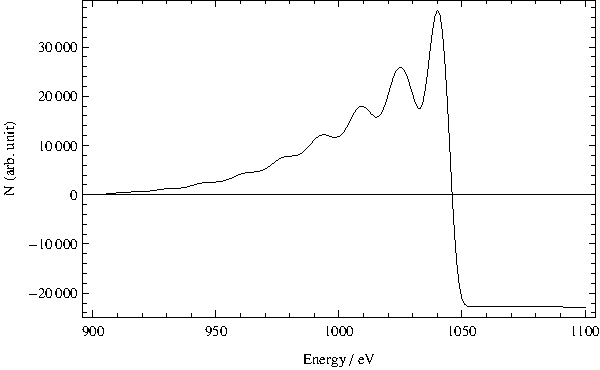
\includegraphics[width=0.48\linewidth]{pic/plasmon1k.pdf}
        \end{tabular}
        \end{center}
        \caption[eel]{
			\small Electron backscatter spectra of Al including additional peaks due to plasmon loss. All values obtained by fitting quadractic functions near the maxima.
			\textbf{(a)} Measurement with electrons of about $170\text{eV}$. Peaks at $(135.84\pm 0.09)\text{eV}$, $(150.52\pm 0.03)\text{eV}$, $(154.55\pm 0.05)\text{eV}$, $(165.65\pm 0.04)\text{eV}$.
			\textbf{(b)} Measurement with electrons of about $1050\text{eV}$. Peaks at $(919.6\pm 6.7)\text{eV}$, $(934.5\pm 5.4)\text{eV}$, $(948.8\pm 1.7)\text{eV}$, $(964.7\pm 1.9)\text{eV}$, $(980.1\pm 1.2)\text{eV}$, $(994.11\pm 0.59)\text{eV}$, $(1009.31\pm 0.26)\text{eV}$, $(1024.96\pm 0.09)\text{eV}$, $(1039.90\pm 0.28)\text{eV}$.
        }
        \label{fig:plas}
\end{figure} 

%TODO letters (a) (b)...

\section{Summary and Discussion}
An aluminium sample was analyzed in a high vacuum chamber with both AES and EELS. The differential Auger electron spectrum was in good agreement with the literature. As the positional offset of the sample was unknown though, it was necessary to recalibrate the spectroscope using one of the measured peaks itself.

Due to the limited resolution of the used apparatus, the KLL spectrum of Aluminium could not fully be observed. The five peaks that were measureable though agree very well with the literature (see section \ref{sec:kll}).

The EELS to measure the energies of plasmons was a full success. Both the energy of the bulk plasmon ($B_1 = (15.3\pm 0.6)\text{eV}$) as well as the energy of the surface plasmon ($S_1 = (11.0\pm 0.2)\text{eV}$) agree with the theory, even though only one surface plasmon was observable.

Despite the good accuracy for the EELS measurements the accuracy for the AES was mediocre at best. While the instruments are precise enough (having negligible error margins compared to the total error), the experimental setup itself causes a lot of noise and is thus the main reason for the (high) errors in the performed experiments. A good place to start improving upon the setup probably is the vacuum pump as well as the positioning of the sample.

\bibliographystyle{unsrt}
\bibliography{FPbib}

\end{document}
